\documentclass[12pt, twoside, openright]{report} % Fuente a 12pt, formato doble página y chapter a la derecha
\raggedbottom % No ajustar el contenido con un salto de página

% MÁRGENES: 2,5 cm sup. e inf.; 3 cm izdo. y dcho.
\usepackage[
a4paper,
vmargin=2.5cm,
hmargin=3cm
]{geometry}

% INTERLINEADO: Estrecho (6 ptos./interlineado 1,15) o Moderado (6 ptos./interlineado 1,5)
\renewcommand{\baselinestretch}{1.15}
\parskip=6pt

% DEFINICIÓN DE COLORES para portada y listados de código
\usepackage[table]{xcolor}
\definecolor{azulUC3M}{RGB}{0,0,102}
\definecolor{gray97}{gray}{.97}
\definecolor{gray75}{gray}{.75}
\definecolor{gray45}{gray}{.45}

% Soporte para GENERAR PDF/A
\usepackage{etoolbox}
\makeatletter
\@ifl@t@r\fmtversion{2021-06-01}%
 {\AddToHook{package/after/xmpincl}
   {\patchcmd\mcs@xmpincl@patchFile{\if\par}{\ifx\par}{}{\fail}}}{}
\makeatother
\usepackage[a-1b]{pdfx}

% ENLACES
\usepackage{hyperref}
\hypersetup{colorlinks=true,
  linkcolor=black, % enlaces a partes del documento (p.e. índice) en color negro
  urlcolor=blue} % enlaces a recursos fuera del documento en azul

% Añadir pdfs como partes del documento
\usepackage{pdfpages}

% Quitar la indentación de principio de los párrafos
\setlength{\parindent}{0em}
\usepackage{multicol}

% EXPRESIONES MATEMÁTICAS
\usepackage{amsmath,amssymb,amsfonts,amsthm}

\usepackage{txfonts} 
\usepackage[T1]{fontenc}
\usepackage[utf8]{inputenc}

% Insertar gráficas y fotos
\usepackage{tikz}
\usepackage{pgfplots}

\usepackage[spanish, es-tabla]{babel} 
\usepackage[babel, spanish=spanish]{csquotes}
\AtBeginEnvironment{quote}{\small}

% diseño de PIE DE PÁGINA
\usepackage{fancyhdr}
\pagestyle{fancy}
\fancyhf{}
\renewcommand{\headrulewidth}{0pt}
\fancyfoot[LE,RO]{\thepage}
\fancypagestyle{plain}{\pagestyle{fancy}}

% DISEÑO DE LOS TÍTULOS de las partes del trabajo (capítulos y epígrafes o subcapítulos)
\usepackage{titlesec}
\usepackage{titletoc}
\titleformat{\chapter}[block]
{\large\bfseries\filcenter}
{\thechapter.}
{5pt}
{\MakeUppercase}
{}
\titlespacing{\chapter}{0pt}{0pt}{*3}
\titlecontents{chapter}
[0pt]                                               
{}
{\contentsmargin{0pt}\thecontentslabel.\enspace\uppercase}
{\contentsmargin{0pt}\uppercase}                        
{\titlerule*[.7pc]{.}\contentspage}                 

\titleformat{\section}
{\bfseries}
{\thesection.}
{5pt}
{}
\titlecontents{section}
[5pt]                                               
{}
{\contentsmargin{0pt}\thecontentslabel.\enspace}
{\contentsmargin{0pt}}
{\titlerule*[.7pc]{.}\contentspage}

\titleformat{\subsection}
{\normalsize\bfseries}
{\thesubsection.}
{5pt}
{}
\titlecontents{subsection}
[10pt]                                               
{}
{\contentsmargin{0pt}                          
  \thecontentslabel.\enspace}
{\contentsmargin{0pt}}                        
{\titlerule*[.7pc]{.}\contentspage}  

% DISEÑO DE TABLAS.
\usepackage{multirow} % permite combinar celdas 
\usepackage{caption} % para personalizar el título de tablas y figuras
\usepackage{floatrow} % utilizamos este paquete y sus macros \ttabbox y \ffigbox para alinear los nombres de tablas y figuras de acuerdo con el estilo definido. Para su uso ver archivo de ejemplo 
\usepackage{array} % con este paquete podemos definir en la siguiente línea un nuevo tipo de columna para tablas: ancho personalizado y contenido centrado
\newcolumntype{P}[1]{>{\centering\arraybackslash}p{#1}}
\DeclareCaptionFormat{upper}{#1#2\uppercase{#3}\par}

% Diseño de tabla para ingeniería
\captionsetup[table]{
  format=hang,
  name=Tabla,
  justification=centering,
  labelsep=colon,
  width=.75\linewidth,
  labelfont=small,
  font=small,
}

% DISEÑO DE FIGURAS.
\usepackage{graphicx}
\graphicspath{{img/}} %ruta a la carpeta de imágenes

% Diseño de figuras para ingeniería
\captionsetup[figure]{
  format=hang,
  name=Fig.,
  singlelinecheck=off,
  labelsep=colon,
  labelfont=small,
  font=small    
}

% NOTAS A PIE DE PÁGINA
\usepackage{chngcntr} % Para numeración continua de las notas al pie
\counterwithout{footnote}{chapter}

% LISTADOS DE CÓDIGO
% soporte y estilo para listados de código. Más información en https://es.wikibooks.org/wiki/Manual_de_LaTeX/Listados_de_código/Listados_con_listings
\usepackage{listings}

% definimos un estilo de listings
\lstdefinestyle{estilo}{ frame=Ltb,
  framerule=0pt,
  aboveskip=0.5cm,
  framextopmargin=3pt,
  framexbottommargin=3pt,
  framexleftmargin=0.4cm,
  framesep=0pt,
  rulesep=.4pt,
  backgroundcolor=\color{gray97},
  rulesepcolor=\color{black},
  %
  basicstyle=\ttfamily\footnotesize,
  keywordstyle=\bfseries,
  stringstyle=\ttfamily,
  showstringspaces = false,
  commentstyle=\color{gray45},     
  %
  numbers=left,
  numbersep=15pt,
  numberstyle=\tiny,
  numberfirstline = false,
  breaklines=true,
  xleftmargin=\parindent
}

\captionsetup[lstlisting]{font=small, labelsep=period}
% fijamos el estilo a utilizar 
\lstset{style=estilo}
\renewcommand{\lstlistingname}{\uppercase{Código}}

\pgfplotsset{compat=1.17} 
%-------------
% DOCUMENTO
%-------------

\begin{document}
\pagenumbering{roman} % Se utilizan cifras romanas en la numeración de las páginas previas al cuerpo del trabajo

%----------
% PORTADA
%---------- 
\begin{titlepage}
	\begin{sffamily}
		\color{azulUC3M}
		\begin{center}
			\begin{figure}[H] % Incluimos el logotipo de la Universidad
				\makebox[\textwidth][c]{
\includegraphics[width=16cm]{Portada_Logo.png}}
			\end{figure}
			\vspace{2.5cm}
			\begin{Large}
				Grado en Ingeniería Informática\\
				2021-2022\\
				\vspace{2cm}
				\textsl{Apuntes}\\
				\bigskip
			\end{Large}
			{\Huge Inteligencia Artificial en las Organizaciones}\\
			\vspace*{0.5cm}
			\rule{10.5cm}{0.1mm}\\
			\vspace*{0.9cm}
			{\LARGE Jorge Rodríguez Fraile\footnote{\href{mailto:100405951@alumnos.uc3m.es}{Universidad: 100405951@alumnos.uc3m.es}  |  \href{mailto:jrf1616@gmail.com}{Personal: jrf1616@gmail.com}}}\\
			\vspace*{1cm}
		\end{center}
		\vfill
		\color{black}
		
\includegraphics[width=4.2cm]{img/creativecommons.png}\\
		Esta obra se encuentra sujeta a la licencia Creative Commons\\ \textbf{Reconocimiento - No Comercial - Sin Obra Derivada}
	\end{sffamily}
\end{titlepage}

%----------
% ÍNDICES
%---------- 

%--
% Índice general
%-
\tableofcontents
\thispagestyle{fancy}

%--
% Índice de figuras. Si no se incluyen, comenta las líneas siguientes
%-
\listoffigures
\thispagestyle{fancy}

%--
% Índice de tablas. Si no se incluyen, comenta las líneas siguientes
%-
\listoftables
\thispagestyle{fancy}

%----------
% TRABAJO
%---------- 

\pagenumbering{arabic} % numeración con números arábigos para el resto de la publicación  


%----------
% COMENZAR A ESCRIBIR AQUÍ
%---------- 

\chapter{Información}

\section{Profesores}
\begin{quote}
	Magistral: Agapito Ledesma, ledezma@inf.uc3m.es, solicitar tutorías por mail con antelación.
	
	Prácticas: Ascensión López Vargas, aslopezv@inf.uc3m.es.
\end{quote}

\chapter{Tema 0: Presentación}

\textbf{Películas sobre IA:} A.I. (Stephen Spielberg), I robot, Terminator (1984) y Morgan (2016).

Sophia, robot social.

Lo que tiene YouTube es datos infinitos, miles de horas por segundo.
WhatsApp hecha para ser comprada al tener todo el nicho de mercado sobre los sistemas de comunicación y “gratis”.
La línea ética es fina en muchas ocasiones, toman muchos datos. La banca y aseguradoras se están beneficiando de la IA para ajustarse o predecir.

GIGO $\rightarrow$ Garbage In Garbage Out (es muy importante la calidad de los datos)

Con el COVID se trató de desarrollar modelos de IA, pero no se tenían apenas datos y menos de calidad.

\section{Tipos:}
\begin{itemize}
	\item Sistemas expertos/difusos, no es uno u otro, sino puntos intermedios. Discursos como poco o mucho.
	\item Redes de neuronas artificiales.
	\item Computación evolutiva, supervivencia del más capaz.
	\item Minoría de datos.
	\item Agentes inteligentes.
	\item Sistemas híbridos.
\end{itemize}

\section{Metodología:}
\begin{itemize}
	\item SPOC (Small Private Online Classes) $\rightarrow$ Teoría
	      \begin{itemize}
		      \item Del tema 2-9
		      \item Videos y lecturas complementarias.
		      \item Test de autoevaluación que se publicaran semanalmente sobre el temario visto.
	      \end{itemize}
	\item Magistral $\rightarrow$ Dudas, Casos prácticos y Test (Wooclap)
	\item Práctica
\end{itemize}

\section{Evaluación}
\begin{itemize}
	\item 60 \% Teoría, nota mínima 4.
	      \begin{itemize}
		      \item 30 \% 2 PEC
		            \begin{itemize}
			            \item Glosario de términos dados en las magistrales
			            \item Preguntas bibliografía
		            \end{itemize}
		      \item 10 \% Seminarios
		            \begin{itemize}
			            \item Presentación
			            \item Memoria
			            \item Coordinación grupal
			            \item Evaluación
		            \end{itemize}
		      \item 10 \% SPOC
		      \item 10 \% i-test en Wooclap
	      \end{itemize}
	\item 40 \% Práctica
	      \begin{itemize}
		      \item 15 \% Prácticas cortas.
		            \begin{itemize}
			            \item Redes de Neuronas Artificiales (2 sesiones).
			            \item Mineria de Datos (2 sesiones).
			            \item Logica difusa (1 sesión).
		            \end{itemize}
		            Evaluación
		            \begin{itemize}
			            \item Planteamiento y desarrollo del problema: 25 \%
			            \item Resultados del problema: 25 \%
			            \item Análisis de resultados y conclusiones: 25 \%
			            \item Presentación: 15 \%
			            \item Contexto de la práctica: 10 \%
		            \end{itemize}
		      \item 10 \% PEC prácticas: Control sobre las practicas (asequible si se han hecho)
		      \item 15 \% Práctica final: Analisis, diseño y contrucción de un sistema basado en tecnicas de IA sobre un tema que nos guste.
		            \begin{itemize}
			            \item Presentación oral (20 \%)
			            \item Presentación del documento (15 \%)
			            \item Introducción y Estado del Arte (15 \%)
			            \item Planteamiento de la solución (20 \%)
			            \item Resultados (10 \%)
			            \item Análisis de Resultados y Conclusiones (20 \%)
		            \end{itemize}
	      \end{itemize}
	      
\end{itemize}

\chapter{Tema 1: Introducción}
\section{Previa}
\subsection{Sistemas inteligentes}
Programas capaces de tomar decisiones, aprender, trabajar de manera autónoma, etc. Hubo un momento que era una palabra comodín, se utilizaba para atraer a la gente al producto, ¿pero realmente lo eran?

\subsection{Inteligencia}
Capacidad de entender, razonar y resolver problemas. Conocimiento, comprensión, acto de entender.

Howard Gardner publicó en 1983 la Teoría de las Inteligencias Múltiples, donde se exponía que no solo hay una manera de inteligencia, sino que dependiendo del ámbito hay un tipo de inteligencia especifica.
\begin{figure}[H]
	\ffigbox[\FBwidth]
	{\caption{Diagrama Inteligencias múltiples}}
	{\def\svgwidth{.8\textwidth}
		\input{img/inteligencia-multiple.eps_tex}}
\end{figure}

\subsection{Inteligencia Artificial}
\subsubsection{Definiciones}
Es una tecnología que parece emular el desempeño humano, típicamente aprendiendo, llegando a sus propias conclusiones, aparentando comprender contenido complejo, participando en diálogos naturales con personas, mejorando el desempeño cognitivo humano o reemplazando personas en la ejecución de tareas no rutinarias.

Disciplina científica que se ocupa de crear programas informáticos que ejecutan operaciones comparables a las que realiza la mente humana, como el aprendizaje o el razonamiento lógico.

La IA no solo es el Deep Learning (Redes de neuronas), sino que hay multitud de áreas.
\begin{figure}[H]
	\ffigbox[\FBwidth]
	{\caption{Mapa de tecnologías IA}}
	{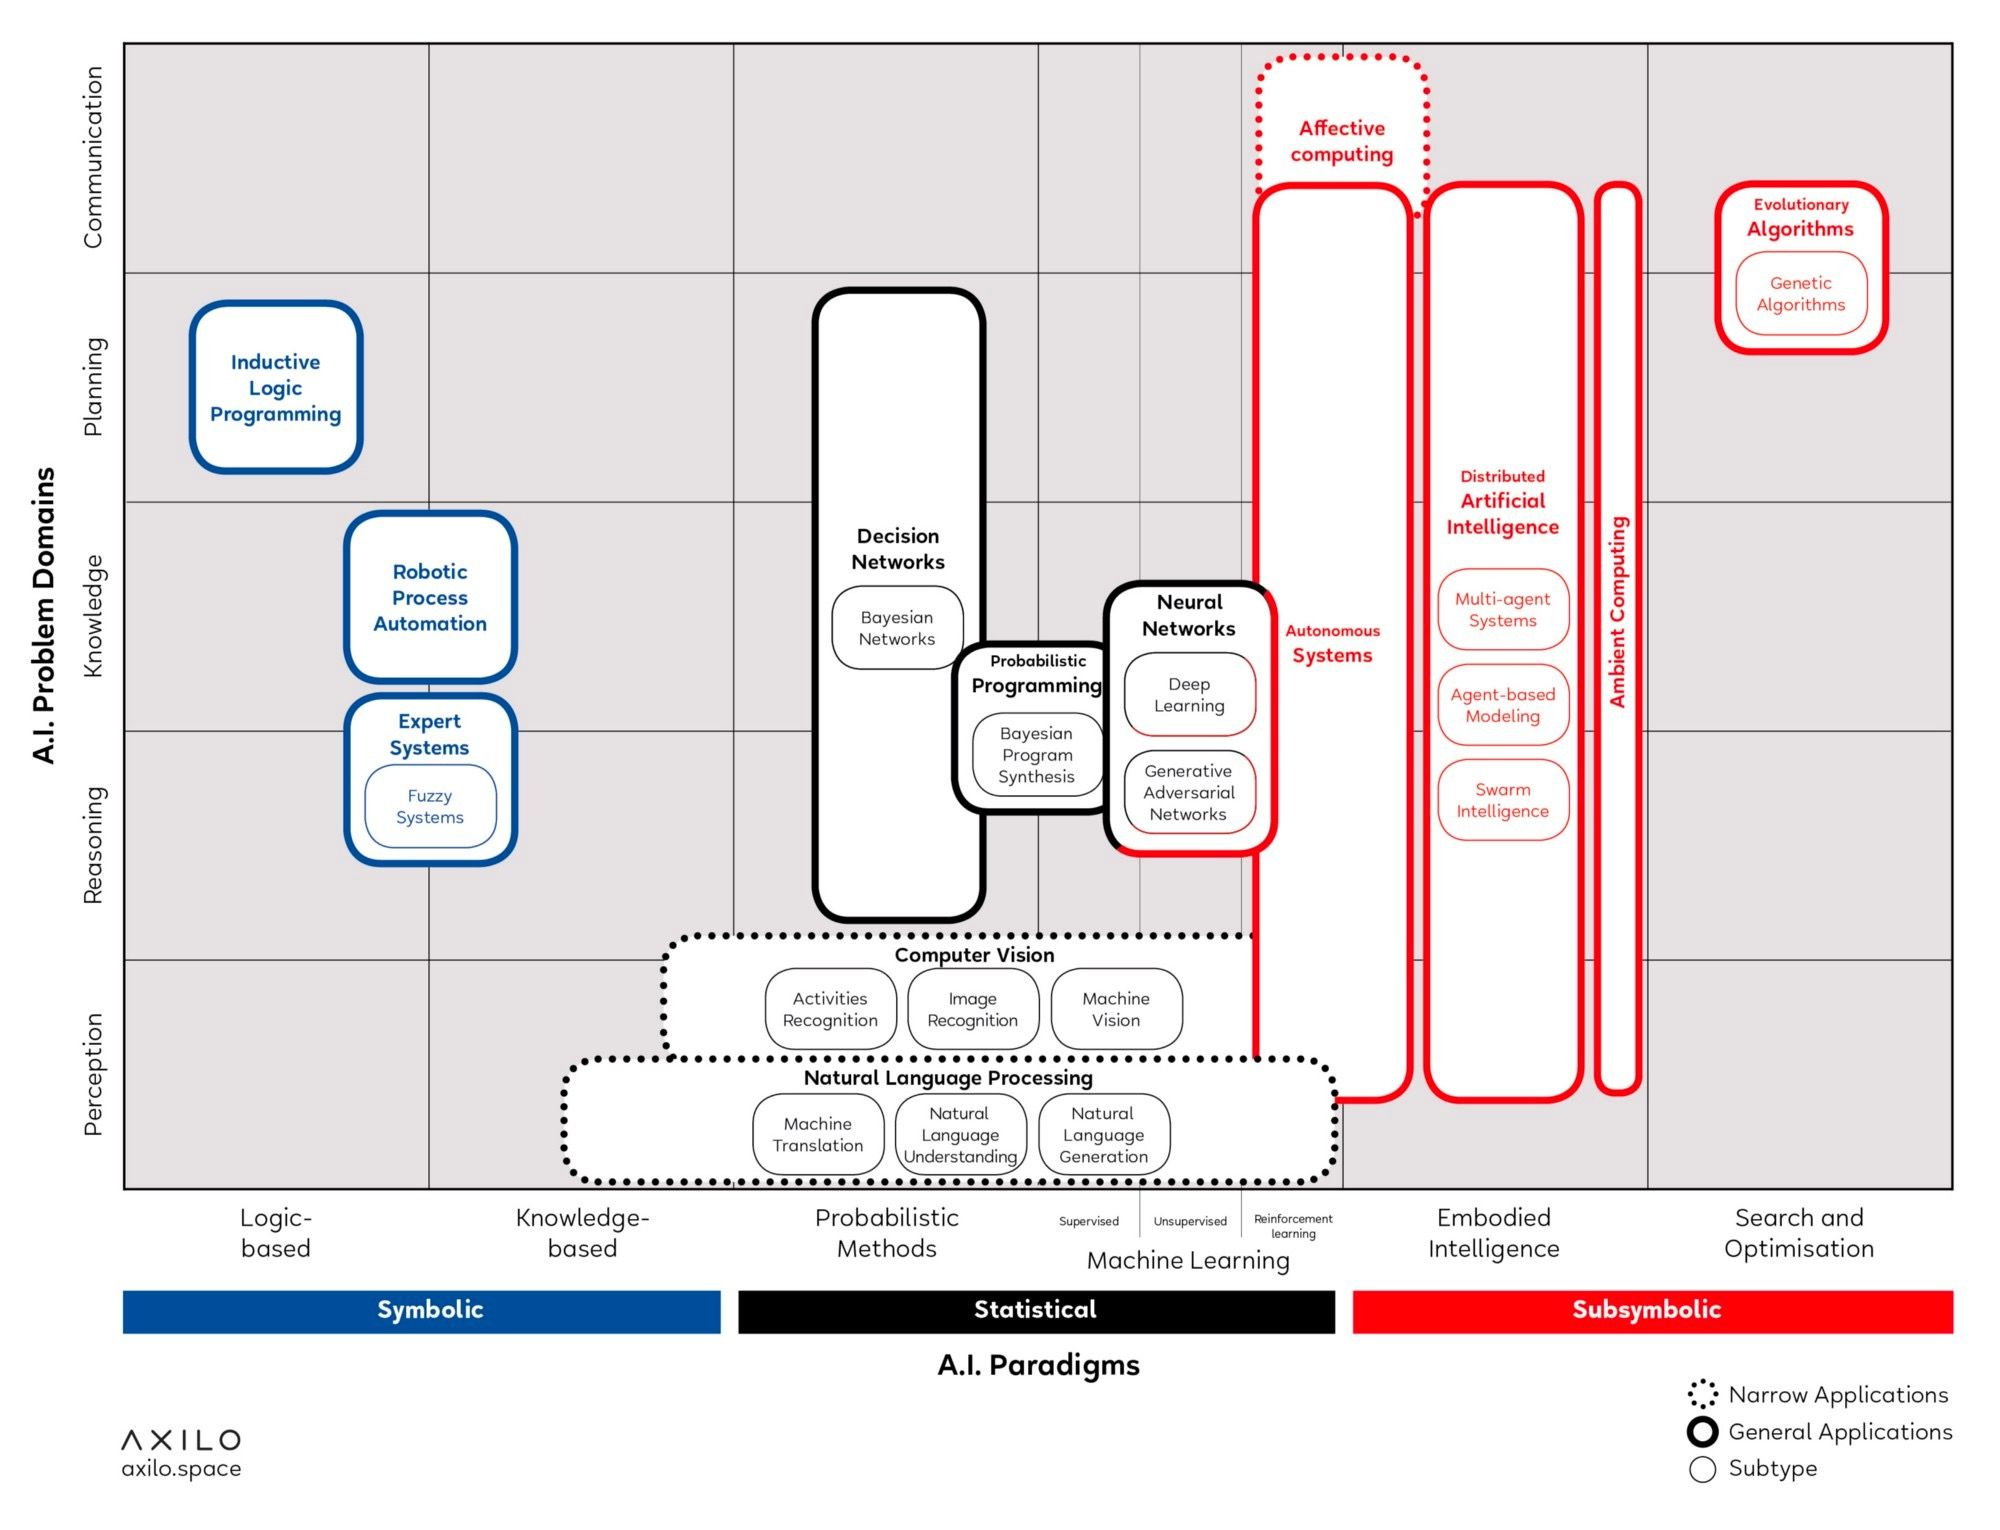
\includegraphics[scale=.23]{areas-ia.jpg}}
\end{figure}

\subsubsection{Historia}
El gran sueño del hombre ha sido siempre crear vida, por lo que hay multitud de proyectos para recrearla en forma de robots como son los geminoids. El problema con los robots que se parecen a los humanos no son sus formas humanoides, sino sus rasgos humanos que provocan del Valle inquietante (provocan incomodidad a las personas).

Por otro lado no solo se trata de que tengan la forma sino también que se comporten como personas, es decir que sean capaces de resolver los problemas de manera parecida siguiendo un razonamiento, de ahí la Inteligencia Artificial.

Alan Turing en 1950 antes de que se acuñase el término de IA dijo:
\begin{displayquote}
	Propongo considerar la siguiente cuestión: ¿pueden pensar las máquinas?
\end{displayquote}

En la cultura popular, literatura y el cine, se ha tratado este tema muchas veces como en Frankenstein, Matrix o Terminator.

En la realidad no hay nada que se parezca a un cerebro humano estamos muy lejos todavía de lograrlo, pero nos permite resolver ciertos problemas. Por ejemplo: Deep Blue de IBM, la RoboCup o Watson de IBM.

Estos últimos tiempos ha podido avanzar tan rápido gracias a la capacidad de cómputo (hardware) y la inmensa cantidad de datos que hay digitalizados y se generan por segundo.

Se han hecho estudios de cuánto tiempo tardará la IA en ser capaz de reemplazar al ser humano en determinadas tareas, como escribir un best-seller, ser cirujano o vendedor de tienda.

\subsection{Ejemplos de su uso}
\begin{itemize}
	\item Google Maps para estimar el tiempo de viaje.
	\item Filtros anti-spam buscando patrones similares a los clasificados como correo basura.
	\item Asistentes como Siri, Alexa o Cortana, eso vienen con un pre-aprendizaje para evitar sesgo.
	\item Antivirus busca patrones de comportamiento.
	\item Reconocimiento facial como en Facebook, Fotos iOS o Google Fotos.
	\item Drones repartidores para suplir la ‘last mile’, capaces de llevar cargas de un punto a otro y recargarse solos.
	\item Sistemas de recomendaciones según el comportamiento del usuario aprende sus gustos.
\end{itemize}

\subsection{Sectores que han adoptado IA mejor}
\begin{itemize}
	\item Alta tecnología y telecomunicaciones.
	\item Automovilística y ensamblado.
	\item Servicios financieros.
	\item Recursos y utilidades.
	\item Entretenimiento y media.
\end{itemize}

\section{Introducción}
En la actualidad se hace algo parecido al clásico ‘Artis Auriferae quam Chemiam vocant’ de la alquimia (química), que quiere decir El Arte de Hacer Oro que era la piedra filosofal de estos expertos, lo que les da poder.

Los profesionales de todas las áreas de la industria y los negocios buscan su particular piedra filosofal, en la actualidad el material valioso es el Conocimiento y el proceso es saber transformar los datos en conocimiento.

Los procesos que emplean los profesionales de negocios son Sistemas Inteligentes que buscan patrones no lineales, son de este tipo porque la mayoría de los problemas son de este tipo. Otro punto que hace complicado encontrar patrones y relaciones en los datos es que los que se encuentren sean útiles.

\subsection{Usos}
\begin{itemize}
	\item Predicción del comportamiento del consumidor, saber que consumen los clientes para de esta manera poder captar su atención y ofrecerles oferta o productos determinados. Actualmente los usuarios buscan un producto más personalizado.
	\item Captura del conocimiento corporativo, recogen el conocimiento de profesionales con experiencia para desarrollar un sistema experto que sea capaces de realizar sus tareas.
	\item Agricultura de precisión, para optimizar el regadío, los fertilizantes o abonos, de esta manera maximizar la producción y agricultura sostenible. Se emplean robots como Wall-Ye que toma medidas de la tierra.
	\item Detección de fraudes, permiten detectar si el usuario se está saliendo de su patrón de comportamiento (conocido por todas sus transacciones), levantar una alerta y bloquear el pago.
	      
	      El factor más importante para combatir el fraude es el Tiempo, por lo que las RNA son una gran herramienta, son capaces de detectar patrones mucho más rápido que una persona y tiene la capacidad de adaptarse.
\end{itemize}
\pagebreak

\section{Contexto}
Todo hoy en día deja un rastro de datos, incluso aunque nosotros no llevemos dispositivos electrónicos hay cámaras, tarjetas, entre muchos otros que son capaces de recoger datos sobre nosotros.

Las grandes empresas (automotrices y financieras) fueron los primeros en darse cuenta de que esos datos son un gran activo que explotar. Los sistemas inteligentes que utilizan buscan relaciones y patrones en grandes cantidades de datos para extraer conocimiento.

Las técnicas más comunes son las Redes de Neuronas dado que hay muchas formas de estas, Algoritmos Genéticos y la lógica difusa. Antes se utilizaba en sistemas no principales, pero hoy en día en el núcleo de la empresa ‘core-business’.

Muchas de estas técnicas están inspiradas en la naturaleza (bioinspiradas), las redes de neuronas en el cerebro, algoritmo evolutivos o inteligencia de enjambre. La pregunta es si ha funcionado en la naturaleza porque no imitarlo para resolver otros problemas.

\subsection{Donde se usa}
\begin{itemize}
	\item \textbf{Banca al por menor:} Evaluación de hipotecas y Predicción de demanda de productos.
	\item \textbf{Planificación:} Localización de minoristas y Distribución de productos.
	\item \textbf{Seguros:} Evaluación de riesgos y Cálculo de primas.
	\item \textbf{Marketing:} Perfiles de clientes y Venta cruzada.
	\item \textbf{Banca de Inversiones:} Predicción de activos y Gestión de cartera.
	\item \textbf{Vigilancia:} Detección de robos internos y Detección de fraudes con tarjetas de crédito.
\end{itemize}

\subsection{Motivación}
Las empresas buscan la reducción de costes, aumentar la calidad del servicio y mejora de las prestaciones del producto.

\subsection{Redes de Neuronas Artificiales}
Es una simplificación de cómo funciona el cerebro humano, su objetivo no es simular el cerebro.

Es un array de números (pesos), que dada una entrada procesa los datos y produce una salida.

\subsection{Algoritmos evolutivos}
Se codifica la solución de un problema y se genera una serie de soluciones que no tienen por qué ser buenas, solo soluciones. Después estas soluciones se mutan para dar lugar a nuevas soluciones que se evaluaran con una función para quedarnos con las mejores, el proceso ser repite mejorando las soluciones progresivamente hasta llegar a la más cercana a la óptima (cuasi óptima).

Están muy orientadas a problemas de optimización.

\section{Características clave}
\begin{itemize}
	\item \textbf{Aprendizaje:} Es la característica más importante de los sistemas inteligentes. Las técnicas actuales difieren mucho de los primeros sistemas expertos, que tenían muy poca capacidad de aprender.
	\item \textbf{Adaptación:} Como todos los negocios y empresas cambian continuamente, los procesos se van quedando obsoletos, por lo que las técnicas tienen que ir evolucionando para seguir siendo útiles. Se podría reentrenar, no dejar de aprender o combinando dos procesos.
	\item \textbf{Flexibilidad:} Las decisiones humanas se caracterizan por una inherente flexibilidad, cada uno percibe las cosas de una manera distinta, pero todos lo hacemos dentro de un rango. Otra manera de expresarla es aun faltando un dato ser capaz de continuar y llevar a cabo el proceso. Los sistemas clásicos funcionan con lógica si/no.
	\item \textbf{Explicación:} Se debe saber cómo se llega a la conclusión del proceso, para poder entender como los realiza y esto permite la interacción el experto que sabrá si lo ha hecho bien. No te fiarías de una máquina que no sabes por qué dice que te tienes que operar.
	\item \textbf{Descubrimiento:} Capacidad de descubrir procesos o relaciones nuevas que no eran conocidas previamente.
	      
	      Los patrones descubiertos deben ser validados por un experto humano.
\end{itemize}

\section{Principales técnicas}
\begin{table}[H]
	\centering
	\caption{Comparativa técnicas IA}
	\resizebox{\textwidth}{!}{%
		\begin{tabular}{|c|c|c|c|c|c|}
			\hline
			Técnica                    & Aprendizaje & Flexibilidad & Adaptación & Explicación                & Descubrimiento \\ \hline
			\begin{tabular}[c]{@{}c@{}}Redes de\\ Neuronas\end{tabular} & ↑↑↑↑↑       & ↑↑↑↑↑        & ↑↑↑↑↑      & \begin{tabular}[c]{@{}c@{}}↑ \\ Suelen ser\\ cajas negras\end{tabular} & ↑↑             \\ \hline
			\begin{tabular}[c]{@{}c@{}}Algoritmos\\ Genéticos\end{tabular} & ↑↑↑↑↑       & ↑↑↑↑         & ↑↑↑↑       & ↑↑↑                        & ↑↑↑↑↑          \\ \hline
			\begin{tabular}[c]{@{}c@{}}Sistemas \\ Borrosos\\ Fuzzy\end{tabular} & ↑           & ↑↑↑↑↑        & ↑          & ↑↑↑                        & ↑              \\ \hline
			\begin{tabular}[c]{@{}c@{}}Sistemas\\ Expertos\end{tabular} & ↑           & ↑            & ↑          & \begin{tabular}[c]{@{}c@{}}↑↑↑↑↑\\ Al estar basado\\ en reglas\end{tabular} & ↑              \\ \hline
		\end{tabular}%
	}
\end{table}
También existen técnicas híbridas.

\section{Actualidad}
La Inteligencia Artificial no reemplaza a las técnicas tradicionales, pero si las enriquece o presenta alternativas.

Algunos sistemas inteligentes producen salidas que pueden ser entendidas por los que toman las decisiones.

La tendencia actual es incorporar los sistemas inteligentes dentro de otras aplicaciones de negocios, actualmente es muy accesible, pero se necesita personal. Utilización en pequeñas y medianas empresas.

Los sistemas híbridos es un área en expansión.

\chapter{Tema 2: Sistemas Expertos}
\section{Introducción}
Estos sistemas surgieron en los 70, pero proliferaron a lo largo de los 80. Se pueden llamar sistemas expertos o sistema basados en conocimiento.

Están dirigidos a resolver tareas en dominios definidos de manera limitada y que requieren conocimiento especializado, de expertos.

Llevan una larga trayectoria, en la que han aparecido numerosas variantes, y se han consolidado en muchos dominios.

\subsection{Dominios y áreas de aplicación}
\begin{multicols}{2}
	\textbf{Dominios}
	\begin{itemize}
		\item Contabilidad
		\item Finanzas
		\item Gerencia
		\item Comercialización
		\item Leyes
		\item Ingeniería
	\end{itemize}
	\columnbreak
	
	\textbf{Áreas de aplicación}
	\begin{itemize}
		\item Resolución de problemas
		\item Tareas de planificación
		\item Tareas en búsqueda
		\item Interpretación
		\item Monitorización
		\item Control
	\end{itemize}
\end{multicols}

\subsection{¿Qué son?}
Son programas de ordenar que exhiben un comportamiento característico de los expertos, personas que dominan un área/materia.

Son sistemas informáticos que utilizan conocimiento experto con el propósito de alcanzar un rendimiento similar al de un experto a la hora de resolver un problema muy bien definido.

Es importante destacar que los Sistemas expertos no sustituyen a los expertos, pero permiten que la experiencia y conocimiento de estos esté disponibles, lo que hace que los no expertos puedan trabajar mejor.

Son la tecnología de Inteligencia Artificial más aplicada hoy en día.

\subsection{¿Cuándo se utilizan?}
Existen unos requerimientos para aplicar un sistema experto, que son:
\begin{itemize}
	\item \textbf{Conocimiento especializado}, que provienen de expertos y libro/textos publicados.
	\item \textbf{Juicio}, la capacidad de tomar decisiones sensatas o llegar a conclusiones razonables, que tenga un criterio.
	\item \textbf{Experiencia}, contar con alguien que sepa resolver el problema para poder seguir adelante.
\end{itemize}

En relación con el problema hay dos características que debe poseer:
\begin{itemize}
	\item El problema debe ser \textbf{heurístico}, que no cuente con una solución algorítmica o al menos no fácil.
	\item El problema debe estar \textbf{bien definido}, tiene que estar claramente identificado.
\end{itemize}
Además, el área de experiencia debe estar muy definido y reconocida a nivel profesional.

Cuando se está desarrollando el sistema se necesita reclutar expertos que deseen cooperar en el desarrollo del sistema. El problema de reclutar al experto es que no quieran porque lo vean como una amenaza que les quite el trabajo.

También hay que tener en cuenta el tamaño y complejidad de la aplicación, deben ir acorde con la organización, de manera que sea manejable en función de los recursos de la organización y contando con el respaldo de la administración. Cuanto más grande y complejo más reglas requerirá.

\section{Conceptos}
\subsection{¿Qué es un sistema experto?}
Feigenbaum; McCorduck y Nii lo definen de la siguiente manera
\begin{quote}
	Los programas de IA que consiguen una capacidad a nivel de expertos en la resolución de problemas mediante la reproducción de un cuerpo de conocimiento se denominan sistemas basados en conocimiento o sistemas expertos.
\end{quote}

Lo que quiere decir que un sistema experto es: Un programa de ordenador que realiza una tarea con el nivel que alcanzaría un experto humano.

Los sistemas expertos intentas incorporar en un programa de ordenador el conocimiento de expertos humanos en un área bien definida.

Un punto clave en estos sistemas es que el dominio debe definirse de una manera limitada, no puede dar respuestas útiles a todas las posibles preguntas. Se limita a un área de conocimiento, como pasa con los expertos humanos.

\textbf{Experto:} Persona que ha desarrollado un alto nivel de habilidades que le permiten hacer juicios en un dominio específico. 

Otro concepto que debemos considerar es la pericia, que es la sabiduría, práctica y experiencia en una ciencia o arte. 

\textbf{Pericia:} Conjunto de capacidades que enfatizan el desempeño de los expertos humanos como extenso conocimiento de dominio, heurísticas que simplifican y mejoran los enfoques para la resolución de problemas, el metaconocimiento y la metacognición. Por último, comportamientos que permiten un mejor desempeño en una tarea determinada.

\subsection{Porque construir un sistema experto?}
Una de las principales razones de las organizaciones es que permite preservar la experiencia, los sistemas expertos almacenan una gran cantidad de conocimiento que pueden poner a disposición de personas con menos experiencia.

Otras razones son: Mejorar la productividad, hacer que la experiencia sea portable u obtener consejo de expertos que de otra manera no sería posible.

\subsection{¿Qué hace falta para construir un sistema experto?}
\begin{itemize}
	\item Lo primero es \textbf{adquirir el conocimiento}, llamado Obtención del conocimiento, que a menudo requiere una serie de entrevistas así como una observación minuciosa del experto mientras lleva a cabo sus tareas.
	\item Una vez hemos adquirido el conocimiento debemos \textbf{representar el conocimiento} de tal manera que pueda ser reutilizado por el ordenador. Existen distintas maneras:
	      \begin{itemize}
		      \item \textbf{Reglas de producción}, que son reglas del tipo Sí … Entonces …
		      \item \textbf{Marcos}, son estructuras de datos que representan situaciones estereotipadas en un dominio mediante el uso de un formalismo baso en conceptos. Se pueden considerar los predecesores de los objetos del paradigma de la Programación Orientada a Objetos.
		      \item \textbf{Redes semánticas}, que utilizan un formalismo basado en relaciones para representar el conocimiento del dominio.
		      \item \textbf{Ontologías}.
	      \end{itemize}
\end{itemize}
La representación más habitual del conocimiento para los sistemas expertos son las reglas de producción. Que tiene la forma de sí se cumple la premisa entonces se realiza la acción.

Los componentes principales para construirlo son:
\begin{itemize}
	\item La \textbf{base del conocimiento}, es una colección de hechos, reglas y procedimientos organizados en esquemas. Contiene toda la información y conocimiento sobre un campo de interés específico.
	\item Un \textbf{motor de inferencia}, cerebro del sistema, contiene las estrategias de inferencia y los controles usados por los expertos para manipular las bases de datos de conocimiento y dominio.
	      
	      Este recibe la consulta mediante la interfaz de usuario y lleva a cabo el razonamiento en la base de conocimiento.
	\item La \textbf{interfaz de usuario}, es un componente orientado a facilitar la comunicación entre el sistema y el usuario.
\end{itemize}
También puede contener un subsistema de explicación, cuya función es explicar el razonamiento llevado a cabo por el sistema experto y justificar las conclusiones alcanzas, y una memoria de trabajo reservada para descripción del problema actual y para registrar los resultados intermedios. 

Otra posible estructura de sistema experto contiene además de los anteriores:
\begin{itemize}
	\item \textbf{Base de datos de dominio}, que contiene la información relevante sobre el dominio o área de interés.
	\item Un \textbf{sistema de gestión de base de datos}, que se encarga de controlar la entrada y gestionar tanto la base de datos de dominio como la base de datos de conocimiento.
	\item Un \textbf{componente de adquisición de conocimiento}, orientado a la extracción y formulación de conocimientos derivados de diversas fuentes, especialmente de expertos. En sistemas más avanzados es capaz de aprender nuevo conocimiento de manera autónoma. Permite la interacción entre el usuario y el sistema.
\end{itemize}

Un concepto importante para estos sistemas es la inferencia.

\textbf{Inferencia:} Es el proceso de encadenar múltiples reglas juntas basadas en los datos de los que se dispone. En un sistema experto lo lleva a cabo el motor de inferencia. Los mecanismos de inferencia más populares para los sistemas basados en reglas son:
\begin{itemize}
	\item \textbf{Encadenamiento hacia delante}, es una búsqueda orientada por los datos, si las cláusulas de la premisa coinciden con la situación actual el proceso intenta afirmar la conclusión.
	\item \textbf{Encadenamiento hacia atrás}, es una búsqueda orientada a objetivos, el proceso comienza con la cláusula de acción de una regla y trabaja hacia atrás a través de una cadena de reglas en un intento de encontrar un conjunto verificable de cláusulas de colisión.
\end{itemize}

\section{Herramientas de desarrollo}
Un proceso tipo para desarrollar un sistema experto incluye:
\begin{itemize}
	\item Adquisición de conocimiento.
	\item Representación del conocimiento.
	\item Selección de herramientas de desarrollo.
	\item Prototipado del sistema.
	\item Evaluación del sistema desarrollado.
	\item Proceso continuo de mejora y mantenimiento.
\end{itemize}
A la hora de seleccionar una herramienta para el desarrollo de sistemas expertos hay que tener en cuenta:
\begin{itemize}
	\item Relación costo/beneficio.
	\item Funcionalidad/Flexibilidad de la herramienta.
	\item Compatibilidad de la herramienta con la infraestructura de información existente, es un aspecto fundamental para facilitar la incorporación del sistema experto a los sistemas actuales de la organización.
	\item Fiabilidad y soporte de proveedor de la herramienta.
\end{itemize}
\subsection{Lenguajes IA}
Para comenzar el desarrollo de un sistema experto se puede hacer desde 0, diseñando y programando los componentes de un sistema experto utilizando el lenguaje de programación de propósito general utilizado en el desarrollo de sistemas basados en inteligencia artificial, como LISP o PROLOG.

Aunque también se puede utilizar lenguajes convencionales, como C, C++ o Java, que permiten dar una mayor flexibilidad a la hora de adaptar el sistema al problema de dominio específico. 

Sin embargo, estos últimos lenguajes no proporcionan una idea de cómo debe ser representado el conocimiento, ni de que mecanismo deben ser diseñados para acceder a la base de conocimiento.

\subsection{Entornos híbridos}
Por otro lado, los entornos híbridos brindan mucha facilidad para la conducción de sistemas expertos, con estas herramientas personas con poca experiencia pueden trabajar con un sistema experto. 

Suelen poseer una Shell de sistema experto que contiene todos los elementos esenciales de un sistema experto, exceptuando el conocimiento específico de dominio, también herramientas para construir interfaces de usuario y más características para facilitar la construcción del sistema experto.

Una Shell es una herramienta específica para sistemas expertos que facilita la implementación de estos sistemas. Además los sistemas expertos llevan mucho tiempo en el mercado, por lo que existen muchos ejemplos. El usuario introduce los parámetros de entrada al sistema y este le da salida para el problema, algunos ejemplos:
\begin{itemize}
	\item \textbf{1st-Class Fusion} brindaba un fácil acceso a la base de conocimiento e incorporaba el algoritmo ID3.
	\item \textbf{Financial Advisor} que analizaba las inversiones de capital activo como equipo e instalaciones. Fue desarrollado 1985.
	\item \textbf{KnowledgePro} es un lenguaje de alto nivel que combina funcionalidades de sistemas expertos e hipertexto. Permitía crear sistemas clásicos de reglas, si-entonces, y leer datos desde base de datos y hojas de cálculo.
	\item \textbf{Leonardo} utilizaba un lenguaje orientado a objetos llamado contract que permitía a los especialistas en marketing analizar su empresa y/o producto con respecto a la competencia.
	\item \textbf{Personal Consultant (PC) Easy} era utilizado para guiar vehículos en almacenes y plantas de manufactura.
\end{itemize}

Una Shell muy usada hoy en día es \textbf{Exsys} desarrollada por Corvid, es una herramienta diseñada para crear sistemas expertos en línea y pensada en usuarios no programadores.
\section{Aplicaciones}
Se aplican en una gran variedad de dominios con el propósito de dar soporte a la toma de decisiones. Se puede ver tanto en el área de los negocios para dar soporte como con usos médicos para el diagnóstico.
\pagebreak

Los primeros sistemas expertos estaban dirigidos al dominio de las ciencias como son:
\begin{itemize}
	\item \textbf{DENDRAL} fue desarrollada por Feigenbaum en 1965 con un razonamiento basado en reglas para deducir la estructura molecular probable de los componentes químicos orgánicos a partir de análisis de químicos conocidos y datos de espectrometrías de masas.
	\item \textbf{MYCIN} desarrollado por investigadores de la Universidad de Stanford está basado en reglas cuya finalidad era el diagnóstico médico de enfermedades bacterianas de la sangre.
	\item \textbf{XCON} es unos de los primeros sistemas expertos aplicados al área de los negocios, desarrollado por Digital Equipment Corporation, es un sistema basado en reglas para determinar la configuración óptima de los sistemas según las necesidades del cliente, era capaz de procesar el pedido en un minuto cuando el equipo de ventas tardaba 25-30 minutos.
\end{itemize}

\textbf{Áreas de aplicación de los SSEE}
\begin{itemize}
	\item \textbf{Finanzas}, que incluye análisis de créditos, evaluación de seguros, prevención de fraudes, evaluación de rendimiento, etc.
	\item \textbf{Procesamiento de datos}, que incluye selección de equipos, evaluación de proveedores y la administración de redes.
	\item \textbf{Marketing}, se aplican en la gestión de la relación con el cliente y para el análisis y planificación del mercado.
	\item \textbf{Recursos humanos}, se utilizan para la evaluación de rendimiento, programación de personal o en la gestión de pensiones.
	\item \textbf{Fabricación}, se utilizan para planificación de producción, la gestión de calidad o el mantenimiento y reparación de equipos.
	\item \textbf{Seguridad}, se han utilizado para la evaluación de amenazas terroristas y la detección de financiación de actividades de este tipo.
	\item \textbf{Automatización de procesos de negocio}, se utiliza en la gestión de call center.
	\item \textbf{Administración de la salud}, se han utilizado para resolver diferentes problemas y la aplicación en la bioinformática.
\end{itemize}
\pagebreak

\textbf{Ejemplos de Sistemas expertos}
\begin{itemize}
	\item \textbf{CoverStory} extrae información de marketing de una base de datos y redacta informes de manera automática.
	\item \textbf{ISIS-11} era utilizado por Westinghouse para programar órdenes de fabricación compleja.
	\item \textbf{CARGEX} es utilizado por Lufthansa para determinar la mejor ruta de envío de mercancía.
	\item \textbf{ACE} utilizado por AT\&T para analizar el mantenimiento de redes telefónicas.
	\item \textbf{AA, Authorizer’s Assistant}, es utilizado por American Express para la utilización de crédito para evitar riesgos a la hora de conceder crédito para disminuir las perdidas.
	\item \textbf{Escape} es utilizado por Ford Motor Company para la autorización y proceso de reclamaciones.
	\item \textbf{GURU} es una herramienta desarrollada por Micro Data Base System para dar soporte a la gerencia y análisis financiero utilizando hojas de cálculo.
	\item \textbf{XSEL} es una versión reescrita de XCON de la compañía Digital Equipment Corporation, su función es dar soporte al equipo de ventas en la configuración de los sistemas de los clientes, paso de 3 horas a 15 minutos.
\end{itemize}

Estos son solo algunos ejemplos, muchas empresas desarrollan sus propios sistemas expertos y no publican sus resultados porque son parte de su core-business.

\section{Beneficios y limitaciones}
\textbf{Beneficios de los Sistemas Expertos}
\begin{itemize}
	\item \textbf{Captura de conocimientos escasos}, se da en los casos en los que los expertos se jubilan o dejan el trabajo, pasando haber insuficientes expertos.
	\item \textbf{Aumento de la productividad y la calidad}, los sistemas expertos son capaces de trabajar más rápido que los humanos y brindar recomendaciones consistentes, reduciendo el orden de magnitud de los errores.
	\item \textbf{Disminución del tiempo de toma de decisiones}, las personas que toman consejo de sistemas expertos pueden tomar decisiones mucho más rápido.
	\item \textbf{Mejora en la resolución de problemas}, los sistemas expertos incorporan conocimiento de múltiples expertos en el proceso de análisis lo que posibilita esta mejora y la Integración de varias opiniones de expertos.
	\item \textbf{Puede trabajar con información incierta o incompleta} como lo haría un ser humano.
\end{itemize}
Estos son solo algunos de los beneficios de utilizar estos sistemas, pero también hay algunas limitaciones.

\textbf{Problemas y limitaciones de los Sistemas Expertos}
\begin{itemize}
	\item \textbf{Falta de disponibilidad del conocimiento}, puede darse el caso de que no se pueda acceder al conocimiento, que no haya expertos en el problema que queremos resolver.
	\item \textbf{Extracción de la experiencia}, es proceso difícil obtener el conocimiento de los humanos.
	\item \textbf{Miedo a compartir conocimiento}, lo sufren algunos expertos por miedo a perder su trabajo y ser remplazados.
	\item \textbf{Dominio estrecho y bien definido.}
	\item \textbf{Vocabulario técnico de los expertos.}
	\item \textbf{Falta de confianza de los usuarios finales en el sistema.}
	\item \textbf{Pueden generar recomendaciones incorrectas.}
\end{itemize}

Investigadores han hecho estudios sobre los factores que determinan el éxito o fracaso de un SSEE, son los siguientes:
\begin{itemize}
	\item \textbf{Contar con un buen gestor.}
	\item \textbf{Participación del usuario y un elemento de formación.}
	\item \textbf{Justificación de la importancia del problema de manera adecuada.}
	\item \textbf{Buena gestión de proyectos.}
	\item Es necesario que el nivel de conocimiento sea lo suficientemente alto.
	\item Debe haber al menos un experto cooperativo.
	\item El problema debe ser principalmente cualitativo.
	\item Debe ser suficientemente limitado el alcance.
	\item La interfaz de usuario debe ser de alta calidad, amigable y capaz de almacenar y manipular el conocimiento.
\end{itemize}

En 1995 se descubrió que solo un tercio de los sistemas expertos que se habían estudiado sobrevivía más allá de los 5 años, por lo general el sistema fallaba debido a problemas administrativos como la falta de aceptación del sistema por parte de los usuarios, la incapacidad de retener a los desarrolladores del sistema, problemas en la fase de transición del desarrollo al mantenimiento (falta de refinamiento del sistema), cambios en la prioridad de la organización. 

Una \textbf{adecuada gestión, desarrollo y despliegue del sistema experto podría resolver la mayoría de estos problemas}.

Hoy en día no se ven muchas publicaciones sobre la aplicación de sistemas expertos, sin embargo como dice \textbf{Richard Barfus “Los sistemas expertos no desaparecieron, sino que fueron encubiertos”}, han evolucionado y se encuentran en sistemas híbridos junto a otros tipos de sistemas inteligentes.

\section{Casos}
\subsection{Caso 1: Cultivo de algodón en Pakistán}
Es un proyecto basado en el Internet de las cosas, IoT, que mediante dispositivos distribuidos y conectados que toman datos nos dan la información sobre los campos.

\textbf{Internet de las cosas (IoT)}: es la red de objetos físicos que contienen tecnología integrada para comunicarse y detectar o interactuar con sus estados internos o el entorno externo. Hoy en día todo está conectado como la lavadora, frigorífico, sensores en el campo, wearable, etc.

Otras tecnologías previas al IoT son:
\begin{itemize}
	\item Radio Frecuency Identification (RFID) es una tecnología que permite localizar objetos en un lugar.
	\item Wireless Sensor Network (WSN) que es una red de objetos interconectados dentro de una misma red para compartir datos.
\end{itemize}

Este proyecto se llevó a cabo en Pakistán porque es un país agrícola, depende mucho de su producción la economía, y se ha enfrentado a perdidas por las siguientes razones.
\begin{itemize}
	\item Siembra retrasada y baja.
	\item calidad de semilla.
	\item Peligros ambientales.
	\item Ataques de insectos y enfermedades.
	\item Riego no planificado y pérdidas de agua.
	\item Cosecha intempestiva.
	\item Uso indebido de fertilizantes e insecticidas.
	\item Falta de maquinaria y equipo.
	\item Mal manejo de cultivos maduros.
\end{itemize}

Por esto surge el proyecto de emplear tecnología para mejorar la producción. Los agricultores son en su mayoría son analfabetos, por lo que se recogerá el conocimiento de expertos y agricultores experimentados para ayudarles, el sistema se consultará a través de una app en distintas lenguas locales.

El sistema tiene como objetivo:
\begin{itemize}
	\item Manejo eficiente de cultivos. Control de riego.
	\item Advertencias y orientaciones medioambientales.
	\item Uso óptimo de fertilizantes, insecticidas y pesticidas.
\end{itemize}

El proceso que se seguirá será primero, Adquisición de conocimiento (desplegar los sensores, datos de plagas, insectos, enfermedades, maleza y entorno de crecimiento), desarrollar el sistema experto en este caso en CLIPS (reglas del tipo IF THEN ELSE) y por último los agricultores consultaran las recomendaciones del sistema.
\begin{itemize}
	\item Síntomas de insectos y recomendaciones de insecticidas.
	\item Síntomas de malezas y recomendación de plaguicidas.
	\item Síntomas de gusanos y recomendaciones de insecticidas.
	\item Programación de riego.
\end{itemize}

Los dispositivos empleados con pequeños y constan de: Sensor de suelo, Sensor de humedad, Sensor de temperatura y Sensores de humedad de la hoja. Todos estos dispositivos están conectados formando una red en la que se van comunicando la información y llega al sistema por el Gateway.

Sensores conectados > Sistema Experto > App móvil

Su estructura consta de Base de conocimiento, motor de inferencia (con agenda), Facilidad de explicación y la interfaz de usuario.

No toda la información viene de los sensores, alguna la da el propio usuario mediante la interfaz, en un futuro con una foto y visión artificial será capaz de reconocerlo por sí mismo.
\pagebreak

Conclusiones
\begin{itemize}
	\item Sistema evaluado entre julio y diciembre de 2015.
	\item Tasa de aceptación del 65 \%, en una encuesta a 100 individuos.
	\item Recomendaciones sobre riego, pestes, insectos y malezas.
\end{itemize}

Trabajos futuros
\begin{itemize}
	\item Despliegue de actuadores en campo, que sean capaces de en función de los parámetros realizarlo ellos mismos.
	\item Mejora de la funcionalidad del servidor.
	\item Despliegue de cámaras en el campo, de esta manera no se mete a mano la información.
\end{itemize}

\subsection{Caso 2: Predicción de inundaciones}
Las catástrofes meteorológicas generan inundaciones, lo que trata este proyecto es de estar prevenidos de estos mediante alertas, ya que son los que generan mayores desastres.

\textbf{Inundación:} es una condición general y temporal de anegación parcial o completa de áreas de tierra normalmente seca por el desbordamiento de aguas continentales o de marea debido a la acumulación o escorrentía inusual y rápida de las aguas superficiales de cualquier fuente.

Datos con los que cuenta
\begin{itemize}
	\item Cantidad de lluvia
	\item Duración de la lluvia
	\item Tasa de cambio en el flujo del río
	\item Nivel del agua del río
	\item Características de la cuenca de drenaje de un río (si el río es capaz de absorber el agua)
	\item Actividades humanas que se desarrolla en el área.
\end{itemize}

Se desarrolló un \textbf{sistema experto basado en reglas de creencias}, cuya estructura es:
\begin{itemize}
	\item Base de conocimiento, cuyo núcleo es la base de reglas de creencia.
	\item Motor de inferencia, realiza el razonamiento probatorio, en vez de encadenamiento hacia delante o atrás.
\end{itemize}

Se utiliza estas reglas para procesar \textbf{varios tipos de incertidumbre} en datos de sensores.
\begin{itemize}
	\item Ignorancia
	\item Incompletitud
	\item Aleatoriedad
	\item Vaguedad
	\item Imprecisión
\end{itemize}

\textbf{Las reglas tiene la forma:} Si lluviaCaida es Media Y DuraciónLluviaCaida es Alta ENTONCES CondiciónMeteorologica es {(Severa, 0), (Moderada, 0.4), (Baja, 0.6)}. Funcionan algo parecido a las reglas difusas.

Estas reglas emplean términos como Alto, Medio o Bajo, además la salida viene dada como la probabilidad de cada uno de los posibles valores de salida.

\textbf{Proceso de inferencia:} Razonamiento Probatorio
\begin{enumerate}
	\item Transformación de entrada
	\item Activación de reglas, se hace match de las reglas para ver cuál es la necesaria.
	\item Actualización de creencias
	\item Agregación de reglas
\end{enumerate}
La inferencia la hacemos de esta manera para tener en cuenta la incertidumbre.

Se van agrupando los factores de entrada generando otros factores que se van relacionando, generando una jerarquía tal que en la parte superior está la salida. La agregación de todas las reglas nos permite saber el nivel de inundación. Por ejemplo el X7 es la salida, pero depende de X8, X9, X10, X11 y X12, que son agrupaciones de entradas.

Mediante la interfaz de entrada, para cada antecedente de las reglas (no son solo las entradas, sino también las agrupaciones intermedias) se definen los intervalos de los términos difusos; alto, medio y bajo, así como el valor por defecto. Lo mismo se realiza para el consecuente.

Este sistema permite actualizar las reglas, de manera que ajusta unos pesos a cada variable de la regla para dar la salida. Se representa el conocimiento de tal manera que tenga la incertidumbre del problema, y con la llegada de las entradas voy actualizando los pesos. Se van agregando las reglas de manera que cuando todas se han lanzado se ha escalado el árbol y se conoce la predicción.

\chapter{Tema 3: Redes de Neuronas}
\section{Introducción}
Las Redes de Neuronas surgen en los años 40 con el objetivo de crear sistemas artificiales que modelen el funcionamiento del cerebro.

A continuación se presentan algunos de los nombres más importantes en la historia de las Redes de Neuronas:
\begin{itemize}
	\item \textbf{McCulloch y Pitts, 1943:} Plantearon el primer modelo matemático de red de neuronas artificiales, se basaron en que las neuronas operan mediante pulsos binarios.
	      
	      Introdujeron el concepto de función de paso por umbral. Permitía simular comportamientos complejos a partir de cálculos muy sencillos, pero carecía de capacidad de aprendizaje.
	\item \textbf{Donald Hebb, 1949:} Se basó en dos conceptos muy importantes y fundamentales que han pasado en el campo de las redes de neuronas y que fueron obtenidos a partir de investigación psicofisiológica.
	      
	      Primera que el aprendizaje se localiza en la sinapsis (conexiones entre neuronas) y segundo la información se representa en el cerebro mediante un conjunto de neuronas que pueden estar activas o inactivas. 
	      
	      Su aportación más importante fue el desarrollo de un procedimiento matemático de aprendizaje que se denomina Aprendizaje en Hebbiano.
	\item \textbf{Frank Rosenblatt, 1957:} Generalizado el modelo de neuronas presentado en el 43 añadiendo aprendizaje y lo llamo Perceptrón. Es la red verdadera red de neuronas más antigua.
	      
	      Intento generalizar el aprendizaje en un modelo en tres niveles y para ello introdujo una capa oculta de neuronas, pero no logro un método matemático para entrenarla. Su perceptrón era capaz de generalizar una vez aprendidos una serie de patrones, pero no era capaz de resolver el problema XOR o problemas de clasificación no separables linealmente.
	\item \textbf{Minsky y Papert, 1969:} Publicaron una crítica muy seria al perceptrón por su naturaleza lineal que lo hacía muy limitado, que produjo una parada muy importante en la investigación denominada Época oscura.
	\item \textbf{Rumelhart, Hinton y McClelland, 1980:} Se creó el grupo de Procesamiento Paralelo Distribuido, dieron lugar a manuales muy influyentes y resurgieron el interés por las redes de neuronas artificiales.
	\item \textbf{John Hopfield, 1982:} Demostró que se puede construir una función de energía para describir la actividad de una red de neuronas monocapa en tiempo discreto. El entrenamiento de una Rede Hopfield consiste en reducir la energía de los estados que la red tiene que aprender.
	\item \textbf{Teuvo Kohonen, 1984:} Comenzó a trabajar en memorias asociativas y matrices de correlación, pero su aportación más importante son los mapas autoorganizativos, un tipo de redes de neuronas no supervisadas que usan una función de vecindad para preservar las propiedades topológicas del espacio de entrada.
	      
	      Está formado por nodo/neuronas, para cada neurona hay un vector de pesos del tamaño de la entrada y su posición en el mapa. La distribución usual es en un espacio de dos dimensiones en forma de rejilla rectangular o hexagonal.
	      
	      También aporto el LVQ un sistema de aprendizaje de carácter competitivo.
	\item \textbf{Stephen Grossberg, 1989:} Propuso junto a Gail Carpenter las ART (Teoría de la Resonancia Adaptativa), se trata de un tipo de redes de neuronas que son capaces de seguir aprendiendo cuando están en uso y son un modelo no supervisado.
\end{itemize}

Se usan de forma extensiva en diferentes problemas reales de muy distintas índoles.

Además, existen investigaciones recientes que han dado lugar a un nuevo paradigma, las redes de neuronas convolucionales o Deep Learning. Modelo propuesto por Yann LeCun en 1982, pero refinado en 2012 por un equipo liderado por Dan Ciresan.

\section{Definición y tipos}
Una \textbf{Red de Neuronas Artificiales} es un modelo (matemático) muy simple del conjunto de neuronas del cerebro. Se trata de conseguir el paso del circuito natural del cerebro al correspondiente circuito artificial o red de neuronas.

Las neuronas del cerebro son lentas en comparación con los circuitos eléctricos ($10^{-3}$ s y $10^{-9}$), pero las naturales realizan computo masivamente paralelo lo que reduce la apariencia de esta lentitud.

Una \textbf{neurona} es una unidad de proceso de 1 o varias entradas y con 1 o varias salidas. En la que se lleva a cabo la suma ponderada de las entradas ($a=x_1*w_1*x_2*w_2$), aplicando un peso a cada una, y se procesa mediante una función de activación ($y=F(a)$) que es la que produce la salida. 

Las señales que llegan a la sinapsis son las entradas y estas señales pueden excitar a la neurona (si es positivo) o inhibirla (si es negativo). Si la suma ponderada supera un umbral se activará, si no permanecerá inactiva. 

Las neuronas se encuentran distribuidas en capas, formadas por al menos 1 neurona, y estas capas están interconectadas, esto da lugar a la Red de Neuronas. La estructura de interconexión recibe el nombre de Arquitectura de la Red o Patrón de interconectividad. Las capas pueden ser: Capa de entrada, Capa oculta o Capa de salida.

Las conexiones del perceptrón están siempre orientadas hacia delante, de esta manera las neuronas de una capa se conectan con todas o algunas de las neuronas de la siguiente capa, el llamado Feedforward.

Para desarrollar una arquitectura de red se debe tener en cuenta el número de capas ocultas y su número de neuronas, que operaciones se pueden hacer en paralelo por las conexiones con la siguiente capa. Este proceso se realiza de manera manual y dependerá del problema a resolver, se está trabajando el diseño automático.

El conocimiento en las RNA se ve representado en el peso de las conexiones entre neuronas, por lo que se aprende modificando estos pesos. Cada modelo dispone de su propia técnica de aprendizaje.

\textbf{Función de activación} es una de las partes más importante de la red, esta nos permite independientemente de la arquitectura aprender relaciones no lineales de los datos. Transforma la correspondencia lineal en no lineal, las funciones más utilizadas son del tipo sigmoide, aunque se puede usar la función escalón.

\textbf{Tipos de aprendizajes}
\begin{itemize}
	\item \textbf{Aprendizaje supervisado:} Un ejemplo es el perceptrón multicapa que es capaz de aprender a partir de un conjunto de ejemplos, pudiendo aproximar funciones no lineales, filtrar ruido en los datos, etc. Este aprendizaje se ha conseguido introduciendo la capa oculta y aplicando los algoritmos de aprendizaje de descenso del error, como backpropagation.
	      
	      Cybenko en 1989 demostró que se puede separar cualquier conjunto de datos aunque tengan relaciones no lineales siempre que se introduzca en el perceptrón una capa oculta sea del tamaño que sea.
	      
	      Las neuronas aparecen en una red agrupadas en las tres capas mencionadas antes:
	      \begin{itemize}
		      \item Capa de entrada, las neuronas reciben información del exterior. No actúan como verdades neuronas, solo reciben las entradas/patrones del exterior y las propagan a la capa siguiente.
		      \item Capas ocultas, son las que realmente realizan el procesamiento de la información, comunican con la entrada y la salida. Realizan el procesamiento no lineal de los patrones recibidos.
		      \item Capa de salida, recibe información de la capa anterior y la envían hacia el exterior proporcionando la respuesta para cada uno de los patrones de entrada.
	      \end{itemize}
	      
	      Para el aprendizaje se proporcionan a la red los datos de entrenamiento, que consisten en patrones de entrenamiento de entrada y salida, en función de la diferencia entre la salida y la salida esperada se van actualizando los pesos ($w_{i+1}=w_i+\Delta w_i$).
	\item \textbf{Aprendizaje no supervisado:} Son capaces de modificar sus parámetros internamente para adaptarse al entorno, descubriendo por si solas características, regularidades o categorías entre los datos de entrada. Proporciona de manera codificada la salida. Las neuronas y sus conexiones muestran cierta capacidad de autoorganización.
\end{itemize}

\section{Aplicaciones}
Las RNA se usan cada vez más en problemas de clasificación, predicción y clustering en ámbitos muy diversos, nosotros en la asignatura trataremos el financiero y empresarial. Algunos ejemplos son:
\begin{itemize}
	\item \textbf{Banco Mello:} Invirtió en un costoso sistema de detección de fraudes y en 6 meses habían costeado el coste del software con el ahorro en esos fraudes detectados.
	\item \textbf{Visa y Mastercard:} Monitorizan diariamente más de 1,2 millones de cuentas gracias a las RNA.
	\item \textbf{Auditorías Internas:} Se utilizan para predicción de ganancias, buscar el momento más adecuado para llevar a cabo una auditoria o gestionar estrategias en determinadas operaciones.
	\item \textbf{Ernst \& Young:} En consultoras de alto nivel, conseguir que gestores financieros mejoren la gestión del capital financiero.
\end{itemize}

En el ámbito empresarial y financiero la ventaja es que se cuenta con muchos datos pertenecientes a la empresa a lo largo del tiempo, con lo que se pueden entrenar y obtener buenos resultados.

Se siguen realizando investigaciones y por lo tanto se producen avances en su propia teoría, aunque tenga un origen antiguo (años 40) hay muchos ámbitos abiertos que estudiar. Algunos de estos ámbitos son:
\begin{itemize}
	\item Los expertos o especialistas que tratan de combinar diferentes redes de neuronas para dar lugar a los llamados \textbf{Ensembles o Conjuntos de Clasificadores}.
	\item El trabajo en \textbf{nuevos algoritmos de aprendizaje} para superar al de retropropagación, incluso en sus versiones más rápidas.
	\item \textbf{Diseño automático de arquitectura}, dado que para utilizar las RNA hay que tener un conocimiento experto, este campo está en constante estudio se trata de poder saltarnos ese conocimiento experto y que un sistema de diseño automático no indique cuál es la red de neurona más adecuada para resolver ese problema.
	\item \textbf{Nuevos modelos de RNA} como son las actuales Redes de Neuronas Convolucionales.
\end{itemize}

\textbf{Ventajas de trabajar con RNA}
\begin{itemize}
	\item Permite alcanzar unos resultados excelentes tanto en clasificación, representación o predicción, con unas tasas de acierto por encima del 98 y 99 \%.
	\item Permiten modelar y predecir comportamientos no lineales a diferencia de los métodos clásicos.
	\item Robustos pueden manejar datos incompletos, con ruido y que contienen incluso ejemplos contradictorios.
	\item Adecuadas en el procesamiento de información en finanzas y negocios.
\end{itemize}

\textbf{Desventajas de las RNA}
\begin{itemize}
	\item Son cajas negras, no son capaces de explicar cuál es la información que les ha conducido a tomar la decisión que proporciona la salida.
\end{itemize}


\section{Casos}
\subsection{Caso 1: Predicción de bancarrotas}
Un problema muy importante para las empresas y entidades financieras. Se emplean redes de neuronas en combinación con otros modelos clásicos para mejorar la predicción, como puede ser el modelo de Altman de predicción de insolvencias.

Mejoran la predicción.

Los modelos existentes son muy complejos, pero aun así incrementó su difusión y su uso según se fueron desarrollando las computadoras y hojas de cálculo.

Tradicionalmente:
\begin{itemize}
	\item \textbf{1966 Beaver:} El primero con el uso de técnicas estadísticas de univarianza. Relaciones financieras para predecir bancarrotas muchos años antes de que estas se produjeran.
	\item \textbf{1969 Altman:} Es el trabajo de referencia. Utilizo análisis mutivarianza.
	\item \textbf{1972 Edmister:} Análisis mutivarianza con análisis de tendencias.
	\item \textbf{1985 Fryman, Altman y Kao:} Utilizaron un algoritmo de particionamiento recursivo, sin embargo son modelos muy complejos que no pueden ser utilizados por personal no formado.
\end{itemize}

\subsubsection{Bankruptcy Prediction using ANN 1995: Dorsey, Edmister y Johnson}
Plantearon el uso de redes de neuronas para la predicción de bancarrotas utilizaron una serie de razones financieras de todas las que hay, que fueron razón de liquidez, solvencia/apalancamiento, endeudamiento y la razón de cobertura.

Estudiaron todas esas razones financieras para predecir bancarrotas del año 1994, estudiando las bancarrotas desde 1981-1991.

Tomaron de entrada 20 empresas de tamaño similar con activos de más de 20 millones, 10 ellas solventes y 10 que habían quebrado. 

Como entradas para la red se calcularon 18 razones financieras y como salida detección de empresas saludables, de riesgo y que quebraran pronto. La salida siendo un valor entre 0 y 1, según un umbral (0.4) marcado indica el estado.

Era capaz de detectar un 100 \% de las que van a quebrar, pero falla prediciendo que no quebraron en un 30 \%.

\subsection{Caso 2: Aplicaciones en Banca}
En este ámbito tiene mucha importancia detectar cuando conceder un crédito o no, detectar fraudes, impagos, etc.

Los analistas de riesgos son los que toman estas decisiones, pero para acceder a los datos que da el banco de España son muy lento, por lo que la aplicación de redes para generar perfiles de solvencia es muy buena.

Las entradas son los valores sobre el cliente (renta, hipoteca, historial de compra, profesión, edad, etc.) y la salida si es solvente o insolvente. Esto se puede generar mediante una red de neuronas, como un perceptrón multicapas, con una capa oculta de tamaño suficiente. 

Con backpropagation podrá ir aprendiendo, como entrada de aprendizaje se utilizará un 60 \% de los datos y se validará con el otro 40 \%. Esto permite que una vez entrenada al recibir un nuevo perfil sea capaz de determinar si es solvente o no.

\subsection{Caso 3: Marketing dirigido por los datos}
Se pueden utilizar redes de neuronas no supervisadas para segmentar clientes, son capaces de encontrar patrones en los datos sin haber sido entrenados para ello de manera más eficiente que los métodos de clustering clásicos.

Lo difícil es encontrar los patrones en los clientes para este marketing.

Ese caso de estudio se trata de una sociedad inmobiliaria con 5 millones de clientes y está usando una campaña por correo para promover un nuevo producto de inversión.

Ha llevado a cabo una primera campaña por correo dirigida a 50000 clientes elegidos al azar, de los que solo ha recibido respuesta positiva de 1000 de ellos (un 2 \%). El objetivo es analizar las respuestas a esta primera campaña para encontrar una manera de enfocar la campaña de forma que las respuestas se dupliquen, pasen a ser un 4 \% y conseguir 40000 nuevos inversores.

Se utilizan como entradas los datos de clientes de la base de datos, se trata de optimizarlo por lo que se usa la antigüedad del cliente (TIMEAC, tiempo que lleva abierta la cuenta en años) y su actividad de cuenta (AVEBAL, balance promedio de cuentas de los últimos 3 meses). La salida es un valor que nos tendrá que permitir diferencias el comportamiento del cliente.

Representando estas variables con respecto a si respondieron o no al correo se puede ver que no hay una clara diferencia, ambas se distribuyen de igual manera.

La puntuación de salida será 1 si contesta y 0 en caso contrario, pero los datos se solapan.

La red utilizada puede ser un perceptrón multicapa con aprendizaje supervisado, ya que la empresa conoce a los clientes y la salida. Tendría 2 neuronas en la capa de entrada, el doble en la capa oculta 4 y la capa de salida con 1 que nos dirá si contestara 1 o no 0.

Para el entrenamiento se dispone de 2000 datos de clientes, 1000 positivos y 1000 negativos.  Cada conjunto se divide en 2 conjuntos de 500. El conjunto de entrenamiento serán un grupo de 500 de los divididos, 500 positivos y 500 negativos. El conjunto de test serán los otros 1000 restantes distribuidos equitativamente.

En el entrenamiento si la red proporciona una respuesta adecuada pasa al siguiente, si se equivoca con respecto a la esperada se ajusta la red para reducir la diferencia. Esto repetido varias veces (100-500) sobre todo el conjunto de entrenamiento provoca que se vaya reduciendo el error hasta un valor aceptable.

Se puede representar de manera tridimensional, en los dos ejes la entrada y la altura la salida de la red, de esta manera podemos distinguir los que responderán y los que no.

Cuando ya está entrenando se le pasan los datos de test y se mide el error cometido por la red. Mediante la Gráfica de ganancia (Acumulado de respuestas vs. Acumulado de NO respuestas) podemos ver por encima de la bisectriz como discrimina la red.

\chapter{Tema 4: Algoritmos Evolutivos}
\section{Introducción}
“Como de cada especie nacen muchos más individuos de los que pueden sobrevivir, y como, en consecuencia, hay una lucha por la vida, que se repite frecuentemente, se sigue que todo ser, \textbf{si varía}, por débilmente que sea, \textbf{de algún modo provecho} para él bajo las complejas y a veces variables condiciones de la vida, tendrá \textbf{mayor probabilidad de sobrevivir y}, de ser así, \textbf{será naturalmente seleccionado}. Según el poderoso principio de la \textbf{herencia}, toda variedad seleccionada tendera a \textbf{propagar} su nueva y modificada forma” \textbf{El origen de las Especies - Charles Darwin 1859}.

Empezamos con una visión general desde el punto de la biología y a partir de esta los conceptos en los que se basa la computación evolutiva, su línea temporal, elementos y características.

\textbf{Evolución:} Serie de transformaciones continuas que va experimentando la naturaleza y los seres que la componen.

\textbf{Evolución biología:} Proceso de transformación de las especies a través de cambios producidos en sucesivas generaciones.

\subsection{Historia de la Evolución}
Hasta el \textbf{siglo XXIII} no se dudaba que la naturaleza fuese inmutable, sin embargo los hallazgos de los investigadores que dieron lugar al descubrimiento de los fósiles contradecían esa naturaleza inmutable.

En el \textbf{siglo XIX, Charles Darwin y Alfred Wallace} tras varias décadas de observación y estudios realizados en distintos lugares del planeta llegaron a una misma conclusión, las especies evolucionaron a lo largo del tiempo. Ambos presentaron conjuntamente sus conclusiones a la comunidad científica en 1858, pero \textbf{Darwin fue quien publicó en 1859 su libro “El origen de las especies”} considerado el libro más influyente en la historia de la ciencia.

Hoy en día la evolución como propiedad de los seres vivos no está puesta en duda, pero si es objeto de debate los mecanismos a través de los cuales tiene lugar dicha evolución. En el siglo XX, en los años 40 se dio forma a lo que hoy se conoce como la \textbf{Teoría de Síntesis Evolutiva Moderna que recoge por un lado la selección natural de Darwin y Wallace y por otro lado la Teoría genética de Mendel base de la herencia genética, la Mutación genética como fuente de variación y la Genética de Poblaciones}.

\subsection{Computación evolutiva}
Los algoritmos evolutivos se basan en la Teoría de Síntesis Evolutiva Moderna, aplica conceptos de esta teoría para obtener una respuesta en cierto tipo de problemas. 

Incorpora tres conceptos básicos de la evolución biológica, \textbf{la Selección, la Herencia y la Variación}. Desde el punto de vista de la computación \textbf{la implementación y combinación de estos tres conceptos da lugar a un algoritmo que supone un proceso de búsqueda}, por esto se utilizan principalmente \textbf{en problemas de diseño y de optimización} cuya respuesta se puede obtener mediante un proceso de búsqueda que no es viable mediante fuerza bruta o la búsqueda heurística.

\subsubsection{Historia de la Computación Evolutiva}
Esta computación empezó en los \textbf{años 50}, durante esta década se generaron prototipos computacionales de los modelos biológicos de la evolución para su análisis y validación.

En los \textbf{años 60} es cuando se traslada a la computación los conceptos de teoría de síntesis evolutiva moderna y se idean y aplican las primeras aproximaciones de los algoritmos evolutivos, dando lugar a los algoritmos genéticos, las estrategias y la programación evolutivas.

Durante 2 décadas, \textbf{los 70 y 80} apenas hubo trabajos que supusieran un avance significativo en este campo.

En los \textbf{años 90} es cuando la comunidad científica se organiza e interactúa con mucho más énfasis, organizando las primeras ediciones de diversas conferencias que hoy en día se siguen celebrando (FOGA, CEC, GECCO, etc.). Estos primeros eventos permitieron poner en común diversas ideas y teorías en busca de un mayor soporte teórico para los distintos enfoques y múltiples aplicaciones generadas hasta el momento.

\subsubsection{Características  y Aplicaciones}
La computación evolutiva es una alternativa viable para dar respuesta a problemas de \textbf{optimización y diseño} donde la elevada complejidad computacional de otros algoritmos impide obtener dicha respuesta en el tiempo requerido, también donde no se puede aplicar una heurística para obtener la solución o solución óptima.

Aplican conceptos biológicos como \textbf{cromosoma, el sobrecruzamiento y mutación del cromosoma y la selección natural}, que permiten obtener \textbf{algoritmos flexibles, fácilmente adaptables y robustos}.

\section{Elementos y características}
\section{Estructura básica}
\section{Taxonomía}
\section{Funciones y operadores}

\end{document}